\documentclass[journal]{IEEEtran}

\usepackage[brazilian]{babel}

\makeatletter
\adddialect\l@BRAZILIAN\l@brazilian
\makeatother


\usepackage[T1]{fontenc}
\usepackage[utf8]{inputenc}
\usepackage{lmodern}

\usepackage{ae}
\usepackage{hyphenat}
\usepackage{fancyhdr}
\usepackage{float}
\usepackage{cite}
\usepackage[pdftex]{hyperref}
\usepackage[pdftex]{color,graphicx}

\usepackage[cmex10]{amsmath}

\usepackage{array}

\usepackage{mdwmath}
\usepackage{mdwtab}
\usepackage{url}
\usepackage{tikz}

\hyphenation{op-tical net-works semi-conduc-tor con-si-de-ram fa-mi-lia-ri-za-ção}
\hypersetup{colorlinks, citecolor=black, filecolor=black, linkcolor=black, urlcolor=blue}

%Algoritmos
\usepackage[portuguese]{algorithm2e}

\begin{document}
\title{Um Estudo da Instabilidade de Saffman-Taylor com Fluido Magnético e, ou Anisotrópico}

% author names and IEEE memberships
% note positions of commas and nonbreaking spaces ( ~ ) LaTeX will not break
% a structure at a ~ so this keeps an author's name from being broken across
% two lines.
% use \thanks{} to gain access to the first footnote area
% a separate \thanks must be used for each paragraph as LaTeX2e's \thanks
% was not built to handle multiple paragraphs

\author{Ataias~Pereira~Reis, Yuri~Dumaresq~Sobral, Francisco~Ricardo~da~Cunha\\Universidade de Brasília\\Departamento de Matemática\\Brasília, Brasil\\ataiasreis@gmail.com}

% The paper headers
\markboth{ProIC, Julho~2013}%
{Shell \MakeLowercase{\textit{et al.}}: Bare Demo of IEEEtran.cls for Journals}

\maketitle


\begin{abstract}
%\boldmath
Criação de algoritmos para resolver equações diferenciais parciais. Uso de diferenças finitas para resolver as equações de Laplace e Poisson, usando método ímplicito e explícito, usando bibliotecas de álgebra linear de código aberto. Análise da diferença de tempo de resolução entre os métodos implícito e explícito. Uso do método iterativo e de resolução direta de sistema linear. 
\end{abstract}
% IEEEtran.cls defaults to using nonbold math in the Abstract.
% This preserves the distinction between vectors and scalars. However,
% if the journal you are submitting to favors bold math in the abstract,
% then you can use LaTeX's standard command \boldmath at the very start
% of the abstract to achieve this. Many IEEE journals frown on math
% in the abstract anyway.

% Note that keywords are not normally used for peerreview papers.
\begin{IEEEkeywords}
Ferrofluidos, Navier~Stokes, EDP, Poisson, Laplace, Diferenças~finitas, Eigen
\end{IEEEkeywords}

% For peer review papers, you can put extra information on the cover
% page as needed:
% \ifCLASSOPTIONpeerreview
% \begin{center} \bfseries EDICS Category: 3-BBND \end{center}
% \fi
%
% For peerreview papers, this IEEEtran command inserts a page break and
% creates the second title. It will be ignored for other modes.
\IEEEpeerreviewmaketitle

\section{Introdução}
A instabilidade de Saffman-Taylor, ou \textit{fingering}, que pode ser visto na Figura \ref{finger}, é um fenômeno que ocorre na superfície de contato entre dois fluidos sob circunstâncias específicas. Esse fenômeno ocorre quando um fluido menos viscoso é injetado para deslocar um outro mais viscoso (na situação inversa, do fluido mais viscoso usado para movimentar o outro, a interface é estavel, não ocorrendo o endedamento). Também pode ocorrer movida pela gravidade, ao invés de injeção de um fluido em outro. Neste caso, a interface separando os fluidos de diferentes densidades está direcionada na horizontal, e o mais pesado está em cima do outro. Este tipo de fenômeno é um problema ocorrente em petrolíferas marítimas. Em tais petrolíferas, ocorre a injeção de água nos tubos de extração de petróleo, no objetivo do óleo subir. Na interface entre água e petróleo, o \textit{fingering} ocorre, originando bolhas de óleo dentro de água, que tem um efeito negativo na extração do petróleo, causando perca de óleo quando a água é jogada fora. Uma maneira de se controlar este fenômeno é usar fluidos magnéticos e a aplicação de campos magnéticos\cite{magnetic_fluids}.
\begin{figure}[!ht]
\centering
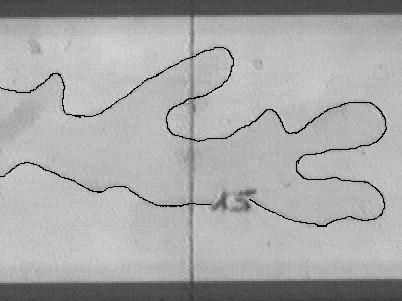
\includegraphics[width=6cm]{figures/fingergel.png}
\caption{Demonstração de fingering\label{finger}}
\end{figure}

O objetivo deste estudo é estudar essa instabilidade por meio de métodos numéricos auxiliados por computador. A equação de Navier Stokes deve ser discretizada e então resolvida numericamente. Ela é uma equação diferencial parcial altamente não-linear e de difícil resolução. No caso da instabilidade de Saffman-Taylor, no qual a fronteira está em movimento, que é a interface entre os dois fluidos, faz-se necessário algoritmos numéricos capazes de lidar com este movimento sem causar complicações extremas que impossibilitem a obtenção de soluções práticas\cite{immersed_boundary_methods}. 

Tais ferramentas numéricas e decisão de métodos/algoritmos a se utilizar são a primeira etapa neste projeto, para então, após se ter tais ferramentas, estudar a física do problema e propor soluções para o problema com a utilização de um ferrofluido. Este relatório mostrará até onde se alcançou na codificação dos algoritmos numéricos para resolução do problema proposto. Iniciou-se com o estudo de equações diferenciais parciais bastante conhecidas, como a equação do Calor, de Laplace, e métodos de solução numérica, especificamente o método de diferenças finitas. Após isso, estudou-se em específico a equação de Navier Stokes\cite{notas_de_aula_john}.

A metologia aqui proposta resume as tarefas realizadas ao longo da execução do projeto:
\begin{enumerate}
  \item[A.] Técnicas de Computação Básica
  \item[B.] Solução da equação de Laplace
  \item[C.] Solução da equação de Poisson
  \item[D.] Solução da equação de Navier Stokes
  \begin{enumerate}
  \item [] Considerações gerais sobre a equação
  \item[1.] Desconsiderando a pressão
  \item[2.] Obtendo a pressão
  \item[3.] Avançando no tempo
  \end{enumerate}
\end{enumerate}
\section{Técnicas de Computação Básica}
Pelo fato da solução numérica da equação diferencial parcial exigir um grande esforço computacional, o tempo de processamento é uma questão fundamental na escolha da linguagem de programação a ser utilizada. De início, a ferramenta e linguagem de programação utilizada era o MATLAB\textregistered. O MATLAB inclui uma infinidade de algoritmos já prontos disponíveis para uso, ferramentas para plotagem de gráficos embutidas, ótimos sistemas de referências de funções, mas tem a desvantagem de consumir muita memória e processamento. O tempo é um fator crítico e o custo computacional de um programa como o MATLAB, sendo executado por muitas horas ou dias, pode ser algo excessivo e, portanto, preferiu-se tomar outro rumo para o desenvolvimento dos códigos.

Tais problemas levaram a uma escolha de uma linguagem de programação compilada e mais rápida, em comparação a uma linguagem interpretada como o MATLAB. A ferramenta escolhida foi o C++. O fato do aluno ter experiência em C inicialmente, aliado ao fato de se haver encontrado uma biblioteca de álgebra linear chamada Eigen\footnote{Eigen: http://eigen.tuxfamily.org/} que evita a necessidade de criação de inúmeros algoritmos básicos, e que é feita em C++, influenciou na escolha de tal linguagem.

A Eigen inclui algoritmos para resolução de sistemas lineares, criação de matrizes e alocação de memória, operações básicas de matrizes, resolução de sistemas de matrizes esparsas e vários outros algoritmos não explorados que estão à disposição, isso tudo de graça, pois é código aberto e gratuito. 

Apesar de se ter escolhido o C++ e a Eigen, isto só não traz todas as ferramentas necessárias ao trabalho em questão. A plotagem de gráficos diretamente em C++ não é algo trivial, não foram encontradas bibliotecas de fácil uso que pudessem ser utilizadas de uma forma tão simples como o MATLAB. Após muita pesquisa, foi decidido utilizar o Python e suas bibliotecas de plotagem de gráficos. Os códigos em C++ passaram a ser compilados não em programas, mas em bibliotecas, e executados de dentro do ambiente Python, que possui poderosos recursos para salvar arquivos, plotar gráficos e com muita documentação disponível.

É utilizado o CMake\footnote{Cmake: http://www.cmake.org/} para criação de Makefiles. Makefiles são arquivos que tem o objetivo de compilar códigos, neles há informação das bibliotecas a qual um programa irá necessitar para ser compilado, localizações de códigos e logicamente o compilador que será utilizado. O CMake simplifica a criação de Makefiles e, por isso, é utilizado. 

Outro programa que se faz uso neste projeto é o git\footnote{Git: http://git-scm.com/}, que é um gerenciador de versões, de forma a sempre se ter as versões antigas dos códigos salvas, e bem organizadas. O projeto tem sido desde certo ponto hospedado num servidor git gratuito, que pode ser obtido facilmente online\footnote{Github projeto: https://github.com/ataias/ff}. Neste site do projeto há um histórico de quase todas as versões dos programas do projeto, e os códigos C++, Python e instruções de como compilar e executar em sistema operacional Ubuntu.
\section{Solução da equação de Laplace}
Primeiramente, o aluno se familiarizou com a resolução de equações diferenciais parciais, estudando em detalhes a solução analítica das equações de Laplace, Poisson, Calor e Onda. O método de resolução aprendido foi o método de Fourier. Tal método consiste na separação de variáveis. Tendo-se uma função incógnita $u(x,y)$, propõe-se uma solução do tipo $H(x)G(y)$ e este termo é então trabalhado na equação diferencial, de forma a obter-se equações diferenciais ordinárias que podem ser resolvidas mais facilmente. As soluções muitas vezes envolvem o uso da série de Fourier, onde partes das EDPs são representadas como uma soma de senos e cossenos, por necessidade pelo uso do método.

Após isso, o primeiro problema proposto foi resolver uma destas equações numericamente, a escolhida foi a equação de Laplace com condições de fronteira de Dirichlet em duas dimensões, num quadrado $1\times 1$. Ela foi escolhida porque é uma EDP muito simples. Verifica-se abaixo o problema:
\begin{eqnarray}
\nabla^2 u=\frac{\partial^2 u}{\partial x^2}+\frac{\partial^2 u}{\partial y^2}=0\label{laplace}\\
u(x,0)=f_1(x),\,u(x,1)=f_2(x)\nonumber \\
\,u(0,y)=g_1(y),\,u(1,y)=g_2(y) \nonumber
\end{eqnarray}

A primeira etapa na resolução numérica desta equação de maneira é discretizá-la, e isto implica em tornar finito o número de pontos em cada dimensão, e representar a equação como operações mais simples e que o computador seja capaz de entender, operações diferentes da derivada, tais como soma, subtração e multiplicação. O método escolhido para realizar a discretização foi diferenças finitas. Este método basicamente faz a seguinte aproximação para a derivada:
\begin{equation}
f'(x)=\lim_{h\rightarrow 0}\frac{f(x+h)-f(x)}{h}=\frac{d}{dx}f(x)\approx \frac{f_i-f_{i-1}}{\Delta x}
\end{equation}
Os valores de $f_i$ são valores discretizados da função $f(x)$, ou seja, $f_i=f(i\Delta x)$. Agora a distância entre dois pontos passa a ser de $\Delta x$. Este valor não está sendo utilizado agora é a distância $\Delta x$. Não é utilizada pelo fato dos valores de $\Delta x$ e $\Delta y$ serem iguais e também pelo fato do lado direito da equação de Laplace ser igual a zero. Caso essas condições fossem diferentes, o problema não se simplificaria. A fórmula para se calcular o espaçamento $\Delta x$ é dada na Equação \ref{delta_x}.

\begin{equation}
\Delta x = 1/(n-1)\label{delta_x}
\end{equation}


Há vários tipos de diferenças finitas: progressivas, regressivas e centrais. Além disso, elas podem envolver mais de dois pontos, de forma a se obter diferentes ordens de erro. O erro também muda de acordo com quão grande é $\Delta x$, que está diretamente ligado ao número de pontos da malha. A malha é uma matriz bidimensional que contém pontos representando posições do espaço. Para resolver a equação de Laplace, utilizou-se diferenças centrais de segunda ordem, cujo erro é da ordem de $\Delta x^2$. A diferença central de segunda ordem é apresentada na equação \ref{diff_central_segunda_ordem}.
\begin{equation}
f''(x)\approx \frac{f(x+\Delta x)-2f(x)-f(x-\Delta x)}{\Delta x^2}\label{diff_central_segunda_ordem}
\end{equation}
Utilizando a discretização da segunda derivada mostrada na Equação \ref{diff_central_segunda_ordem} na equação de Laplace, obtém-se a Equação \ref{laplace_discreta_zero}, que é a equação de Laplace discretizada. Note-se que $\Delta x=\Delta y$ e que a variável $x$ varia de acordo com o índice $i$ e a variável $y$ de acordo com o índice $j$.
\begin{equation}
\frac{u_{i+1j}+u_{i-1j}+u_{ij+1}+u_{ij-1}-4u_{ij}}{\Delta x^2}=0 \label{laplace_discreta_zero}
\end{equation}
Reordenando essa equação álgebrica para encontrar o valor de $u_{ij}$:
\begin{equation}
  u_{ij}=\frac{u_{i+1j}+u_{i-1j}+u_{ij+1}+u_{ij-1}}{4} \label{laplace_discreta}
\end{equation}

A Equação \ref{laplace_discreta} está na forma explícita, na qual um ponto central é obtido diretamente a partir dos pontos adjacentes. No entanto, quando a equação é aplicada ao ponto central, ele influencia no cálculo de outros, que faz com que esta fórmula deva ser aplicada muitas vezes, até se alcançar a convergência de todos os pontos do domínio. A convergência é a aproximação do resultado, quando os valores da malha alcançam valores praticamente estacionários, mudando muito pouco, a solução é óbtida.

Caso essa equação é aplicada a todos os pontos do domínio, se nota um problema, pois ela requere pontos adjacentes em todo local no qual ela é aplicada. Por isso, além da equação, necessita-se das condições de contorno para o problema, onde-se são determinados os valores nas fronteiras do domínio, de forma direta ou indireta, dependendo se as condições são de Dirichlet, Neumann ou uma mistura. No caso atual, as condições são de Dirichlet, que indica o valor de forma direta que a fronteira deve ter. O domínio escolhido é um quadrado, como já mencionado, e na Figura \ref{malha_poisson} tem-se o exemplo de uma malha 6x6.

\begin{figure}[!ht]
\centering
\begin{tikzpicture}
%grid
\draw (0,0) grid +(5,5);

%axes
\draw[->] (0,0) -- (xyz cs:x=0, y=5.2);
\draw (0,5.5) node {$y,j$};

\draw[->] (0,0) -- (xyz cs:x=5.2,y=0);
\draw (5.6,0) node {$x,i$};
\draw (-0.18,-0.18) node {$O$};

\draw (0.3,0.2) node {$x_{00}$};
\draw (0,0) circle (2pt);

\draw (5.3,5.2) node {$x_{55}$};
\draw (5,5) circle (2pt);

\draw (1.3,2.2) node {$x_{12}$};
\draw (1,2) circle (2pt);
\end{tikzpicture}
\caption{Malha padrão para discretizar Laplace e Poisson\label{malha_poisson}}
\end{figure}
Cada cruzamento de linha indica um ponto no domínio, e a Equação \ref{laplace_discreta} será aplicada em quase todos estes pontos, com exceção dos de fronteira, cujo valor da função em tais é determinada pelas condições de Dirichlet. Pontos de fronteira são aqueles que estão sobre uma coluna ou linha dos extremos da matriz.

Pelo fato do método ser iterativo, com um \textit{loop} sendo repetido muitas vezes, até a convergência ser obtida, é natural escolher um método de parada. Isto poderia ser: (1) escolher um tempo limite de execução, (2) ver a diferença entre duas matrizes após uma iteração completa em seus pontos internos, para analisar se a diferença entre elas é desprezível e se indica convergência, ou ainda (3) pode-se calcular os valor da equação de Laplace em cada ponto interno, que seria o melhor a se fazer, e analisar se a equação está dentro de uma faixa de erro desejada. No Algoritmo \ref{algo_laplace_iter}, é apresentada a formulação inicial utilizada.

\begin{algorithm}
\SetKwInOut{Input}{input}\SetKwInOut{Output}{output}
\Input{Matriz com as condições de contorno de tamanho $n\times n$}
\Output{Matriz com cada ponto interno satisfazendo a equação de Laplace e a fronteira igual à entrada}
\BlankLine
$STOP=0$\;
$err \leftarrow 10^{-6}$\;
\While{$STOP \neq 1$}{\label{InRes1}
$u^{\textrm{old}}\leftarrow u$\;

\For{$i\leftarrow 1$ \KwTo $n-2$}{
\For{$j\leftarrow 1$ \KwTo $n-2$}{\label{forins}
$u_{ij}\leftarrow (u_{i+1j}+u_{i-1j}+u_{ij+1}+u_{ij-1})/4$\;
}
}
$ERROR\leftarrow Norma(u^{\textrm{old}}-u)$\;

\If{$ERROR < err$}{
$STOP\leftarrow1$\;
}
}

\caption{Resolvendo a equação de Laplace Iterativamente}\label{algo_laplace_iter}
\end{algorithm}

O método de resolução apresentado no Algoritmo \ref{algo_laplace_iter} foi o primeiro a ser estudado por simplicidade. Este método é chamado de Gauss-Seidel. Note que o valor de cada ponto no método é obtido diretamente dos pontos adjacentes e, portanto, se faz necessária uma resolução iterativa. Isso tem um custo de processamento razoável, no qual o tempo aumenta grandemente conforme o número de pontos $n$ escolhido. Os resultados que mostram essa relação com o número de pontos são mostrados nas Figuras \ref{pontos_vs_tempo_1th} e \ref{pontos_vs_tempo_4th}. Tendo em vista uma resolução mais rápida e direta, pode-se utilizar o método implícito.

% Pontos vs Tempo de Cálculo - 1 Thread  
\begin{figure}[ht!]
\centering
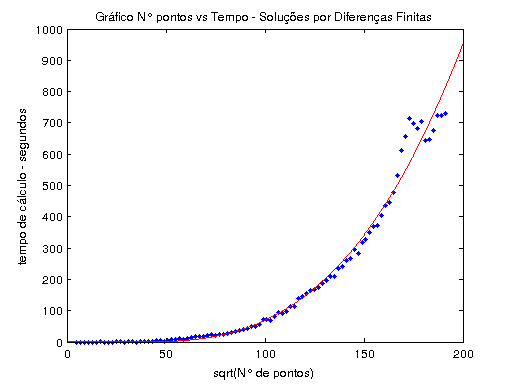
\includegraphics[width = 0.4\textwidth]{figures/problema01_m1/03.png}
\caption{Pontos vs Tempo de Cálculo - 1 thread - Método Explícito\label{pontos_vs_tempo_1th}}
\end{figure}

Nas Figuras \ref{pontos_vs_tempo_1th} e \ref{pontos_vs_tempo_4th} tem-se uma visão geral do tempo que o programa criado consome para resolver a equação de Laplace com condições de Dirichlet, pelo método explícito iterativo. Os conjuntos de pontos obtidos nos dois últimos gráficos mencionados foram aproximados por polinômios cúbicos. A diferença entre os dois se observa no tempo de cálculo quando o número de pontos em cada dimensão, $n$, ultrapassa um valor em torno de 100. Pelo fato de serem polinômios cúbicos, ambos crescem muito rápido com o número de pontos. O cálculo com 4 threads foi mais rápido pelo fato de se estar utilizando mais poder de processamento do computador nos cálculos.

As Figuras \ref{malha5x5_1th}, \ref{malha40x40_1th}, \ref{malha200x200_1th} e \ref{malha500x500_1th} são um conjunto de resultados da equação de Laplace com condições de fronteira de Dirichlet, resolvidas pelo método iterativo explícito, com uso de 1 thread, enquanto as Figuras \ref{malha5x5_4th}, \ref{malha40x40_4th}, \ref{malha200x200_4th} e \ref{malha500x500_4th} são soluções do mesmo problema com o uso de 4 threads do computador. As condições de contorno em todas são as mesmas em todas essas figuras, como se pode notar pelo formato similar de cada uma das soluções. Os lados tem valores de condições de Dirichlet que são $u(x,0)=0$, $u(x,1)=50$, $u(0,y)=75$ e $u(1,y)=100$. 

Note que que conforme se aumenta o número de pontos, o gasto computacional chega a ser excessivo, conforme se observa no tempo gasto para cada solução. O tempo, em segundos, sem nenhuma casa decimal depois da vírgula, está disponível para observação nas descrições das Figuras \ref{malha5x5_1th} a \ref{malha500x500_4th}.

% Pontos vs Tempo de Cálculo - 4 threads
\begin{figure}[ht!]
\centering
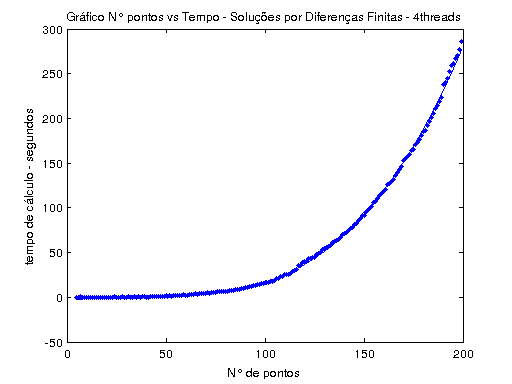
\includegraphics[width = 0.4\textwidth]{figures/problema01_m1/08.png}
\caption{Pontos vs Tempo de Cálculo - 4 threads - Método Explícito\label{pontos_vs_tempo_4th}}
\end{figure}

% Cálculo da Malha 5x5 - 1 thread
\begin{figure}[ht!]
\centering
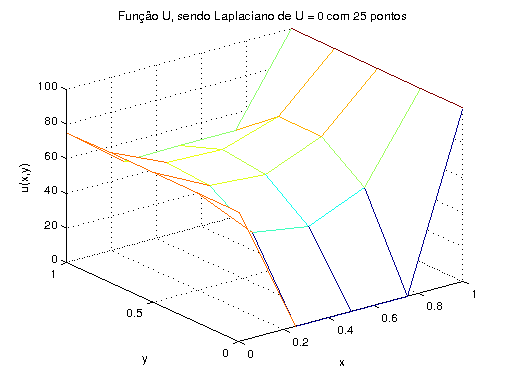
\includegraphics[width = 0.4\textwidth]{figures/problema01_m1/01.png}
\caption{Malha 5x5 - 1 thread - Tempo: 0s - Método Explícito\label{malha5x5_1th}}
\end{figure}

% Cálculo da Malha 5x5 - 4 threads
\begin{figure}[ht!]
\centering
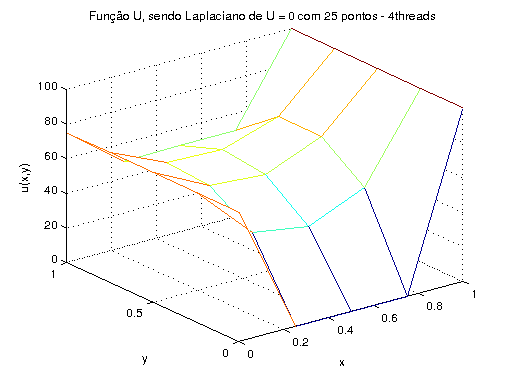
\includegraphics[width = 0.4\textwidth]{figures/problema01_m1/09.png}
\caption{Malha 5x5 - 4 threads - Tempo: 0s - Método Explícito\label{malha5x5_4th}}
\end{figure}

% Cálculo da Malha 40x40 - 1 thread
\begin{figure}[ht!]
\centering
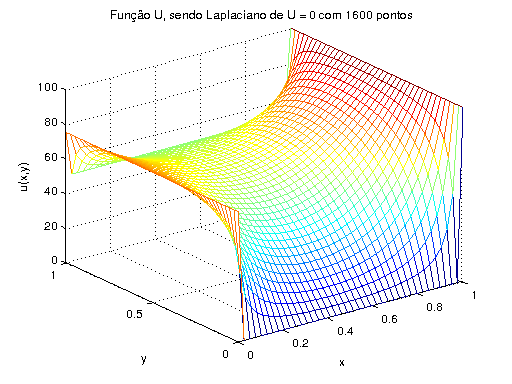
\includegraphics[width = 0.4\textwidth]{figures/problema01_m1/04.png}
\caption{Malha 40x40 - 1 thread - Tempo: 2s - Método Explícito\label{malha40x40_1th}}
\end{figure}

% Cálculo da Malha 40x40 - 4 threads
\begin{figure}[ht!]
\centering
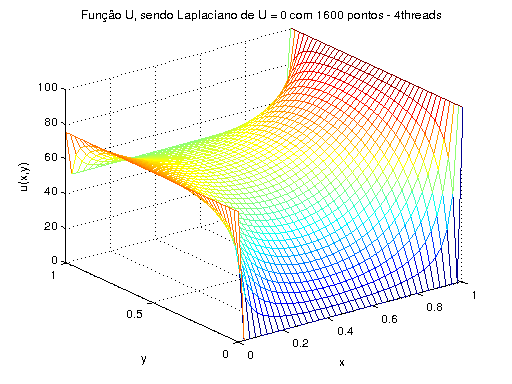
\includegraphics[width = 0.4\textwidth]{figures/problema01_m1/10.png}
\caption{Malha 40x40 - 4 threads - Tempo: 0s - Método Explícito\label{malha40x40_4th}}
\end{figure}

% Cálculo da Malha 200x200 - 1 thread
\begin{figure}[ht!]

\centering
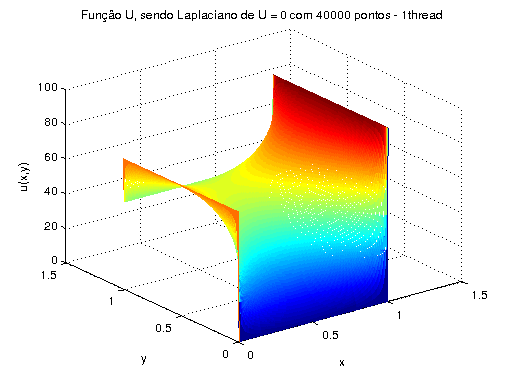
\includegraphics[width = 0.4\textwidth]{figures/problema01_m1/13.png}
\caption{Malha 200x200 - 1 thread - Tempo: 1235s - Método Explícito\label{malha200x200_1th}}
\end{figure}

% Cálculo da Malha 200x200 - 4 threads
\begin{figure}[ht!]

\centering
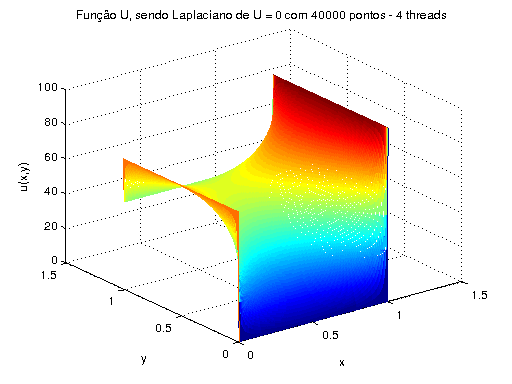
\includegraphics[width = 0.4\textwidth]{figures/problema01_m1/14.png}
\caption{Malha 200x200 - 4 threads - Tempo: 274s - Método Explícito\label{malha200x200_4th}}
\end{figure}

% Cálculo da Malha 500x500 - 1 thread
\begin{figure}[ht!]

\centering
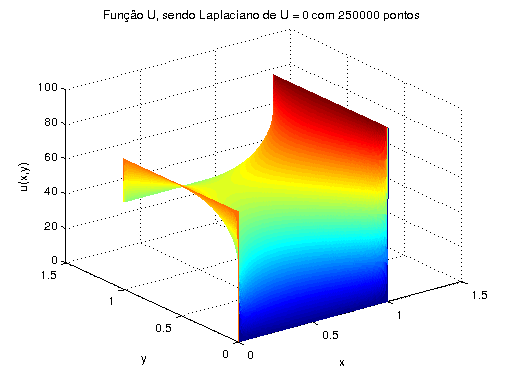
\includegraphics[width = 0.4\textwidth]{figures/problema01_m1/06.png}
\caption{Malha 500x500 - 1 thread - Tempo: 36083s - Método Explícito\label{malha500x500_1th}}
\end{figure}

% Cálculo da Malha 500x500 - 4 threads
\begin{figure}[ht!]

\centering
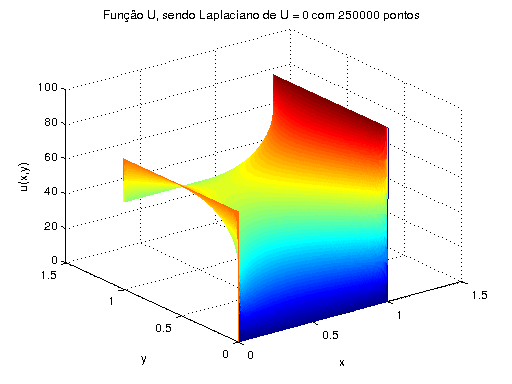
\includegraphics[width = 0.4\textwidth]{figures/problema01_m1/15.png}
\caption{Malha 500x500 - 4 threads - Tempo: 9610s - Método Explícito\label{malha500x500_4th}}
\end{figure}

O uso de paralelismo ocorreu por causa do elevado custo computacional para malhas maiores e, sabendo-se que computadores atuais tem múltiplos threads, fez-se uso deste recurso para analisar a relação entre tempo e número de pontos\footnote{Pontos: o eixo de número de pontos nos gráficos do método explícito na verdade é a ordem da malha, que é a raiz quadrada do número de pontos.} com paralelismo em ação. Resultados similares foram obtidos no caso de múltiplos threads, mudando somente o tempo necessário para cada solução, e podem ser vistos nas Figuras \ref{malha5x5_4th}, \ref{malha40x40_4th}, \ref{malha200x200_4th} e \ref{malha500x500_4th}.

No caso do método ímplicito, utilizando matrizes esparsas, os resultados foram espantosamente mais rápidos. Na maior malha que foi calculada no método explícito, foram gastas 10h\footnote{36083s} no cálculo com 1 thread e 2h40min\footnote{9610s} no cálculo com 4 threads. No método ímplicito com matrizes esparsas, o mesmo resultado foi obtido em menos de 1min. O método ímplicito não é utilizado em Navier Stokes devido ao problema da pressão nesta equação ter fronteiras de Neumann, e o método ímplicito se torna muito complicado. Os resultados para Poisson são similares, só mudando o tempo no caso do método explícito.

Outra forma de se resolver o mesmo problema é substituir na Equação \ref{laplace_discreta_zero} os índices $(i,j)$ por números de fato, obtendo várias equações, e isolando na parte da direita os termos de fronteira. Assim, para um sistema $n\times n$, dos $n^2$ pontos da malha dos índices $(0,0)\rightarrow (n-1,n-1)$, $(n-1)^2$ pontos são internos, correspondendo aos índices de $(1,1)\rightarrow (n-2,n-2)$. As Equações \ref{first_implicit} a \ref{last_implicit} foram obtidas para um sistema $5\times 5$.

\begin{eqnarray}
u_{12}+u_{21} -4u_{11}& = & -u_{01}-u_{10} \label{first_implicit} \\
u_{11}+u_{22}+u_{31}-4u_{21}& =& -u_{20} \\
u_{21}+u_{32}-4u_{31}&=&-u_{41}-u_{30} \\
u_{22}+u_{13}+u_{11}-4u_{12}&=&-u_{02} \\
u_{32}+u_{12}+u_{23}+u_{21}-4u_{22}&=&0 \\
u_{22}+u_{33}+u_{31}-4u_{32}&=&-u_{42} \\
u_{23}+u_{12}-4u_{13}&=&-u_{03}-u_{14} \\
u_{33}+u_{13}+u_{22}-4u_{23}&=&-u_{24} \\
u_{23}+u_{32}-4u_{33}&=&-u_{43}-u_{34} \label{last_implicit}
\end{eqnarray}

O conjunto das Equações \ref{first_implicit} a \ref{last_implicit} é um sistema linear, e é possível representá-lo na forma matricial $Ax = b$. O que torna este problema interessante é que a matriz $A$ e $b$ tem padrões muito bem definidos. A matriz $A$ toma a seguinte forma:
\[ \left( \begin{array}{ccccccccc}
-4 & 1 & 0 & 1 & 0 & 0 & 0 & 0 & 0 \\ % 1
1 & -4 & 1 & 0 & 1 & 0 & 0 & 0 & 0 \\ % 2
0 & 1 & -4 & 0 & 0 & 1 & 0 & 0 & 0 \\ % 3
1 & 0 & 0 & -4 & 1 & 0 & 1 & 0 & 0 \\ % 4
0 & 1 & 0 & 1 & -4 & 1 & 0 & 1 & 0 \\ % 5
0 & 0 & 1 & 0 & 1 & -4 & 0 & 0 & 1 \\ % 6 
0 & 0 & 0 & 1 & 0 & 0 & -4 & 1 & 0 \\ % 7
0 & 0 & 0 & 0 & 1 & 0 & 1 & -4 & 1 \\ % 8
0 & 0 & 0 & 0 & 0 & 1 & 0 & 1 & -4 \\ % 9
\end{array} \right)\]

Observando o padrão de formação da matriz $A$ pentadiagonal e sabendo-se também obter o vetor de valores conhecidos $b$, tem-se um sistema linear para obter os pontos internos $x$. A solução é $x=A^{-1}b$.

Como se nota, a resolução é muito mais direta, mas o algoritmo para se resolver este sistema linear pode ser muito mais complexo. Mas há um problema para este método, que um sistema pode ficar extremamente grande com um $n$ relativamente pequeno, tão grande, ao ponto de necessitar de mais memória do que o computador tem. Isso se resolve utilizando matrizes esparsas, que só salvam na memória elementos diferentes de zero. A matriz $A$ é uma matriz esparsa, na qual a maioria de seus elementos é igual a 0. Também utilizaram-se métodos prontos para resolução de sistemas esparsos provenientes da Eigen.
\section{Equação de Poisson}

A equação de Poisson é muito similar a de Laplace, mas com uma diferença, que é a de haver uma função forçamento existente no lado direito da equação.
\begin{equation}
  \nabla^2 u=\frac{\partial^2 u}{\partial x^2}+\frac{\partial^2 u}{\partial y^2}=f(x,y)\label{poisson}
\end{equation}

Este foi o segundo problema proposto, e o fato de ter essa função $f(x,y)$ complica o problema porque muita coisa que antes era desconsiderada com o $0$ na equação de Laplace não é mais ignorado, mas sim levado em consideração. No caso explícito, tem-se a seguinte discretização obtida:
\begin{equation}
u_{ij}=\frac{1}{4}[(u_{i+1j}+u_{i-1j}+u_{ij+1}+u_{ij-1})-\Delta x^2 f_{ij}] \label{poisson_discreta}
\end{equation}

O algoritmo iterativo para este caso é o mesmo anterior, substituindo a equação \ref{laplace_discreta} por \ref{poisson_discreta} no algoritmo.

Para o caso implícito, o problema é muito similar, bastando mudar o vetor $b$, que passa a apresentar termos $\Delta x^2 f_{ij}$.

A equação de Poisson realmente complicou quando se preparou o algoritmo numa versão mais similar àquela que é utilizada em Navier Stokes. Esta versão resolve o problema de Poisson com as quatro fronteiras com condições de Neumann, isto é:
\begin{equation}
\frac{\partial u}{\partial n} = f
\end{equation}

Isto resulta em maior processamento devido à esta equação gerar condições na fronteira que não são inicialmente fixas, mas que também são incógnitas. O problema foi resolvido e é apresentado na seção de resultados.

A Equação \ref{poisson_problem_solved_neumann} foi resolvida. Note que se trata de uma equação de Poisson com condições de contorno de Neumann.
\begin{eqnarray}
\nabla^2 u = 1 \label{poisson_problem_solved_neumann}\\
\frac{\partial u}{\partial n}=0\,\textrm{na fronteira, exceto}\\
\frac{\partial u(x,0)}{\partial y}=2x
\end{eqnarray}

As soluções da Equação \ref{poisson_problem_solved_neumann} são apresentadas nas Figuras \ref{poisson_neumann_contorno} e \ref{poisson_neumann}.
\begin{figure}[ht!]
\centering
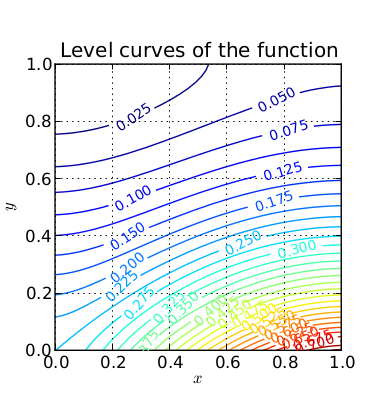
\includegraphics[width = 0.25\textwidth]{figures/poisson_neumann_02.png}
\caption{Poisson com 4 fronteiras de Neumann - Linhas de contorno\label{poisson_neumann_contorno}}
\end{figure}

\begin{figure}[ht!]
\centering
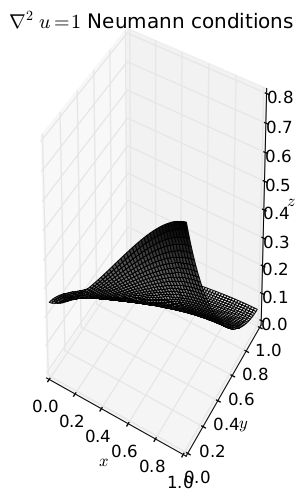
\includegraphics[width = 0.4\textwidth]{figures/poisson_neumann_01.png}
\caption{Poisson com 4 fronteiras de Neumann\label{poisson_neumann}}
\end{figure}

\section{Equação de Navier Stokes}
\subsection*{Considerações gerais}
Após resolver-se as equações de Laplace e Poisson com condições de Dirichlet, pelos métodos explícito e implícito, tem-se já uma base para partir para a próxima etapa: Navier Stokes. Essa equação tem muitas complicações, e está levando ainda certo tempo para ter-se um programa que a resolva, e esteja de fato livre de bugs. A complexidade do programa é muitas maior, tem várias etapas, e tem ainda uma evolução no tempo que não foi lidada nos problemas anteriores. A equação de Navier Stokes é a seguinte:

\begin{eqnarray}
\rho\left( \frac{\partial \textbf{v}}{\partial
t}+\textbf{v}\cdot\nabla\textbf{v}\right)=-\nabla
p+\mu\nabla^2\textbf{v}+\textbf{f} \label{ns}\\
 \nabla\cdot \textbf{v}=0 \label{divergente_zero}
\end{eqnarray}

A discretização não é simples e é um pouco diferente das que foram feitas anteriormente. Em primeiro lugar, tem-se de saber que a discretização de Navier Stokes que será feita aqui é a fórmulação em variáveis primitivas. Isso quer dizer que o problema será trabalhado com as variáveis originais de velocidade $u$, $v$ (em $x$ e $y$) e pressão $p$. Outra forma de resolver é usando uma formulação com a vorticidade, que não será trabalhada aqui.

No que se aprendeu lendo sobre tal formulação do processo de resolução em variáveis primitivas, sabe-se que utilizando uma malha como a da Figura \ref{malha_poisson}, ocorrem modos espúrios de pressão que causam um perfil de velocidades que contém oscilações não esperadas no resultado do problema. O resultado, obtido com tal malha, desta forma, não é satisfatório, e para resolver este problema usa-se uma malha escalonada.

A malha escalonada é uma malha na qual valores guardados num ponto se referem à informação em um outro ponto, próximo. No ponto $P=(i,j)$ são salvos cinco valores: força horizontal, força vertical, pressão, velocidade horizontal e vertical. Essas são representadas pelos símbolos $f_x$, $f_y$, $p$, $u$ e $v$. Um elemento da malha escalonada é representado na figura a seguir, na qual as forças não estão mostradas, mas elas são localizadas nas mesmas posições que as velocidades.

\begin{figure}[!ht]
\centering
\begin{tikzpicture}
\draw (0,0) rectangle (2,2);
\draw (1.35,1.2) node {$p_{i+\frac{1}{2}j+\frac{1}{2}}$};
\draw[->] (1,-0.2) -- (1,0.2);
\draw (1,-0.3) node {$v_{i+\frac{1}{2}j}$};
\draw[->] (-0.2,1) -- (0.2,1);
\draw (-0.5,1.3) node {$u_{ij+\frac{1}{2}}$};
\draw (1,1) circle (2pt);

\draw (0,0) circle (2pt);
\draw (-0.25,-0.25) node {$ij$};
\end{tikzpicture}
\caption{Elemento de malha escalonada}
\end{figure}

Diferente dos problemas de Laplace e Poisson, no qual um elemento $u_{ij}$ que estava salvo no computador na posição $ij$ realmente é o elemento $u_{ij}$, agora o elemento $u_{ij}$ salvo na memória do computador é fisicamente o elemento $u_{ij+\frac{1}{2}}$, enquanto o elemento $v_{ij}$ se refere ao elemento $v_{i+\frac{1}{2}j}$. De maneira similar ocorre para as forças. Para a pressão, $p_{ij}$ corresponde ao ponto $p_{i+\frac{1}{2}j+\frac{1}{2}}$. Isso influencia diretamente na discretização, e na posterior criação dos gráficos.

Uma malha escalonada completa é apresentada na Figura a seguir:

\begin{figure}
\centering
\tikzstyle{help lines}+=[dashed]% aaarghhh!!!
\begin{tikzpicture}
%axes
\draw[->] (0,5) -- (xyz cs:y=6);
\draw (0,6.3) node {$y(j)$};
\draw[->] (5,0) -- (xyz cs:x=6);
\draw (6.5,0) node {$x(i)$};
\draw (-0.18,-0.18) node {$O$};
%grid
\draw[style=help lines] (-1,-1) grid +(7,7);
\draw (0,0) grid +(5,5);
%internal p points
\foreach \x in {0.5,1.5,2.5,3.5,4.5}
  \foreach \y in {0.5,1.5,2.5,3.5,4.5}
  {
  \fill (canvas cs:x=\x cm,y=\y cm) circle (2pt);
}
%External p points
\foreach \x in {0.5,1.5,2.5,3.5,4.5}
  \draw (\x,-0.5) circle (2pt);
\foreach \y in {0.5,1.5,2.5,3.5,4.5}
  \draw (5.5,\y) circle (2pt);
\foreach \y in {0.5,1.5,2.5,3.5,4.5}
  \draw (-0.5,\y) circle (2pt);
\foreach \x in {0.5,1.5,2.5,3.5,4.5}
  \draw (\x,5.5) circle (2pt);
%Internal Horizontal Velocities Points
\foreach \x in {-1.2,-0.2,0.8,1.8,2.8,3.8,4.8}
  \foreach \y in {0.5,1.5,2.5,3.5,4.5}
  {
  \draw[->] (\x,\y) -- (\x+0.4,\y);
}
%External Horizontal Velocities Points
\foreach \x in {-.2,0.8,1.8,2.8,3.8}
  \draw[->] (\x,5.5) -- (\x+0.4,5.5);
\foreach \x in {-.2,0.8,1.8,2.8,3.8}
  \draw[->] (\x,-.5) -- (\x+0.4,-.5);
%Internal Vertical Velocities Points
\foreach \x in {0.5,1.5,2.5,3.5,4.5}
  \foreach \y in {-1.2,-0.2,0.8,1.8,2.8,3.8,4.8}
  {
  \draw[->] (\x,\y) -- (\x,\y+0.4);
}
%External Vertical Velocities Points
\foreach \y in {-0.2,0.8,1.8,2.8,3.8}
  \draw[->] (5.5,\y) -- (5.5,\y+0.4);
\foreach \y in {-0.2,0.8,1.8,2.8,3.8}
  \draw[->] (-.5,\y) -- (-.5,\y+0.4);
\end{tikzpicture}
\caption{Malha escalonada. Círculos são pontos internos e de fronteira enquanto circunferências indicam fronteira imaginária adicionada\label{malha_escalonada}}
\end{figure}

Na malha escalonada da Figura \ref{malha_escalonada}, tem-se ainda uma nova adição: uma fronteira imaginária. Quando se discretiza a equação de Navier Stokes, faz-se ainda necessários outros pontos além do internos e fronteira. As equações apresentadas são discretizadas em domínios similares ao de cima, onde a única coisa que muda é o tamanho do domínio, que pode ser maior.

O problema de Navier Stokes é trabalhado em três etapas principais:

\begin{enumerate}
  \item Desconsiderando a pressão
  \item Obtendo a pressão
  \item Avanço no tempo
\end{enumerate}

Inicia-se agora a descrição da metodologia empregada em tais etapas.

\subsection{Desconsiderando a pressão}
A primeira etapa consiste literalmente de desconsiderar a pressão. Há um termo de pressão na Equação de Navier Stokes (eq. \ref{ns}) que é o termo $\nabla p$, chamado de gradiente de pressão. Elimina-se ele da equação e a partir dessa simplificação, faz-se a discretização da equação. Pelo fato da malha ser escalonada, termos de velocidade estão em pontos diferentes da malha, e há momentos nos quais é necessário elementos de velocidade que não estão salvos na malha, fazendo-se necessária obter uma média de velocidades próximas para obter as velocidades necessárias na discretização.
 
\begin{eqnarray}
\textbf{v}_{ij}^s=(u_{i+1j}+u_{i-1j}+u_{ij+1}+u_{ij-1})\textbf{i} 
\nonumber \\+(v_{i+1j}+v_{i-1j}+v_{ij+1}+v_{ij-1})\textbf{j}\\
\textbf{v}_{ij}^t=0.25(u_{ij}+u_{i+1j}+u_{i+1j-1}+u_{ij-1})\textbf{i}\nonumber \\
+0.25(v_{ij}+v_{i-1j}+v_{i-1j+1}+v_{ij+1})\textbf{j}
\end{eqnarray}
\begin{eqnarray}
u_{ij}^{*}&=&\left[\frac{\mu}{\rho}\left(\frac{u_{ij}^s-4u_{ij}}{\Delta
x^2}\right)+\frac{1}{\rho}f_{x,ij}\right] + u_{ij}\nonumber \\
&-&\left[u_{ij}\frac{u_{i+1j}-u_{i-1j}}{2\Delta
x}-v_{ij}^t\frac{u_{ij+1}-u_{ij-1}}{2\Delta x}\right]\Delta t
\end{eqnarray}

\begin{eqnarray}
v_{ij}^{*}&=&\left[\frac{\mu}{\rho}\left(\frac{v_{ij}^s-4v_{ij}}{\Delta
x^2}\right)+\frac{1}{\rho}f_{y,ij}\right] + v_{ij}\nonumber \\
&-&\left[u_{ij}^t\frac{v_{i+1j}-v_{i-1j}}{2\Delta
x}-v_{ij}\frac{v_{ij+1}-v_{ij-1}}{2\Delta x}\right]\Delta t
\end{eqnarray}

Com isto, tem-se:
\[\textbf{v}^{*}=(u^*,v^*)\]

As equações para $u_{ij}^{*}$ e $v_{ij}^{*}$ são utilizadas para obter a solução de velocidades da equação de Navier Stokes sem a pressão, portanto, não é a solução real, mas está relacionada com a solução.

\subsection{Obtendo a pressão}
A forma de obter a pressão é utilizando as Equações \ref{ns} e \ref{divergente_zero}. Primeiro é obtido o divergente da Eq. \ref{ns} e então, utilizando a Equação \ref{divergente_zero}, se simplifica a equação obtida, obtendo-se o seguinte:

\begin{equation}
\nabla^2 p = \frac{\rho}{\Delta t} \nabla\cdot \textbf{v}^*=\frac{\rho}{\Delta t} 
\left( \frac{\partial u^*}{\partial x}+\frac{\partial v^*}{\partial y} \right) \label{poisson_ns}
\end{equation}

O termo da direita na equação acima será chamado de $DIV$, e é discretizado na equação seguinte:

\begin{equation}
DIV_{ij}=\frac{\rho}{\Delta t}\left( \frac{u_{i+1j}^*-u_{ij}^*}{\Delta x}+\frac{v_{ij+1}^*-v_{ij}^*}{\Delta x}\right)
\end{equation}

A equação que estamos tratando é a de Poisson, e resultará na pressão desejada para resolvermos o problema de Navier Stokes. A Equação \ref{poisson_discreta} é usada para pontos internos da malha. Já para a fronteira, a situação muda em relação à anterior. A partir da equação de Navier Stokes podem ser obtidas as condições de contorno para a pressão. Veremos que tais condições são todas de Neumann, fazendo com que não haja uma única solução de pressão, mas como na equação de Navier Stokes só aparece gradiente de pressão, qualquer solução de pressão pode ser usada para então obter esse gradiente. Destrinchando a Equação \ref{ns} em duas coordenadas, tem-se:

\begin{eqnarray}
\frac{\partial u}{\partial t}+u\frac{\partial u}{\partial x}+v\frac{\partial
u}{\partial y}=-\frac{1}{\rho}\frac{\partial p}{\partial
x}+\nu\left(\frac{\partial^2 u}{\partial^2 x}+\frac{\partial^2 u}{\partial^2
y}\right)+f_x\\
\frac{\partial v}{\partial t}+u\frac{\partial v}{\partial x}+v\frac{\partial
v}{\partial y}=-\frac{1}{\rho}\frac{\partial p}{\partial
y}+\nu\left(\frac{\partial^2 v}{\partial^2 x}+\frac{\partial^2 v}{\partial^2
y}\right)+f_y
\end{eqnarray}

Se fizermos uma análise dos pontos na parede da esquerda ou
direita, e aplicarmos as condições de impenetrabilidade e não-deslizamento, que
dizem que $u=0$ e $v=0$ na parede, temos a simplificação da equação, pois vários
termos se tornam zero. As equações para as duas paredes verticais é a seguinte:
\begin{equation}
\frac{\partial p}{\partial x}\Bigg|_{\textrm{parede}}=\rho\nu\frac{\partial^2
u}{\partial x^2}\Bigg|_{\textrm{parede}}+\rho f_x \label{parede_vertical_pressao}
\end{equation}

Para as paredes que ficam na horizontal tem-se:
\begin{equation}
\frac{\partial p}{\partial y}\Bigg|_{\textrm{parede}}=\rho\nu\frac{\partial^2
v}{\partial y^2}\Bigg|_{\textrm{parede}}+\rho f_y \label{parede_horizontal_pressao}
\end{equation}

As discretizações das Equações \ref{parede_vertical_pressao} e \ref{parede_horizontal_pressao} devem ser feitas considerando-se a malha escalonada, da forma como os dados são salvos no computador. O seguinte esquema mostra a origem $O$ do nosso domínio e o ponto no computador que representa a origem imaginária $x_{00}$:

\begin{figure}
\centering
\tikzstyle{help lines}+=[dashed]% aaarghhh!!!
\begin{tikzpicture}
%grid
\draw[style=help lines] (-1,-1) grid +(7,7);
\draw (0,0) grid +(5,5);

%axes
\draw[->] (0,0) -- (xyz cs:x=0, y=6.2);
\draw (0,6.5) node {$y$};

\draw[->] (0,0) -- (xyz cs:x=6.2,y=0);
\draw (6.6,0) node {$x$};
\draw (-0.18,-0.18) node {$O$};

\draw[->] (-1,-1) -- (xyz cs:x=-1, y=6.2);
\draw (-1,6.5) node {$j$};

\draw[->] (-1,-1) -- (xyz cs:x=6.2, y=-1);
\draw (6.7,-1) node {$i$};

\draw (-1.3,-1.3) node {$x_{00}$};
\draw (-1,-1) circle (2pt);

\draw (0.3,0.2) node {$x_{11}$};
\draw (0,0) circle (2pt);

\draw (5.3,5.2) node {$x_{66}$};
\draw (5,5) circle (2pt);

\draw (6.3,6.2) node {$x_{77}$};
\draw (6,6) circle (2pt);

\draw (1.3,2.2) node {$x_{23}$};
\draw (1,2) circle (2pt);
\end{tikzpicture}
\caption{Mostra dos índices dos pontos do domínio e pontos imaginários}
\end{figure}
Esta malha é mostrada como na figura acima porque em C++ não é possível ter elementos de matrizes com índices negativos, como em Fortran. Discretizando as equações e isolando os termos da fronteira imaginária, que se deseja obter, tem-se o seguinte:
\begin{eqnarray}
p_{i-1j}|_{i=1}&=&p_{ij}-\frac{\mu}{\Delta x}\left(2u_{ij}-5u_{i+1j}+4u_{i+2j}-u_{i+3j}\right)\nonumber\\ & & -\rho\Delta x f_{ij}\\
p_{i+1j}|_{i=n}&=&p_{ij}+\frac{\mu}{\Delta x}\left(2u_{ij}-5u_{i-1j}+4u_{i-2j}-u_{i-3j}\right)\nonumber\\ & &+\rho\Delta x f_{ij}\\
p_{ij-1}|_{j=1}&=&p_{ij}-\frac{\mu}{\Delta x}\left(2v_{ij}-5v_{ij+1}+4u_{ij+2}-u_{ij+3}\right)\nonumber\\& &-\rho\Delta x f_{ij}\\
p_{ij+1}|_{j=n}&=&p_{ij}+\frac{\mu}{\Delta x}\left(2v_{ij}-5v_{ij-1}+4u_{ij-2}-u_{ij-3}\right)\nonumber\\& &+\rho\Delta x f_{ij}
\end{eqnarray}

Tais equações devem então ser utilizadas no algoritmo para resolver a equação de Poisson, lembrando que essas condições são de Neumann, e então a fronteira não é fixa, mas irá variar até o momento que o algoritmo iterativo utilizado convergir.
\subsection{Avanço no tempo}
Agora faz-se a relação entre a velocidade obtida ignorando-se a pressão com o gradiente da pressão obtida no item anterior para então obter-se o próximo passo de tempo da velocidade. Finalmente, tem-se: 

\begin{equation}
\frac{\textbf{v}^{n+1}-\textbf{v}^*}{\Delta t}=-\frac{1}{\rho}\nabla p
\end{equation}

Expandindo para as equações escalares, tem-se:
\begin{eqnarray}
u^{n+1}=u^*-\frac{\Delta t}{\rho}\frac{\partial p}{\partial x}\\
v^{n+1}=v^*-\frac{\Delta t}{\rho}\frac{\partial p}{\partial y}
\end{eqnarray}
Basta discretizar os termos das derivadas parciais agora:

\begin{eqnarray}
p_{x,ij}=\frac{p_{ij}-p_{i-1j}}{\Delta x}\\
p_{y,ij}=\frac{p_{ij}-p_{ij-1}}{\Delta x}
\end{eqnarray}

E finalmente tem-se a solução para o tempo $n+1$ a partir do tempo passado $n$:

\begin{eqnarray}
u^{n+1}=u^*-\frac{\Delta t}{\rho}p_x\\
v^{n+1}=v^*-\frac{\Delta t}{\rho}p_y
\end{eqnarray}
Cada uma das varíaveis acima é uma matriz. Com isso, tem-se as fórmulas necessárias para resolver a equação de Navier Stokes. No entanto, mais processos são necessários computacionalmente, é necessário escolher uma boa condição de parada para as etapas que consideram convergência, trabalhar com arquivos para salvar os resultados, entre outras coisas, que realmente complicam a solução do problema.

Não há resultados para a equação de Navier Stokes, pois está muito complicado descobrir os bugs ainda existentes no programa. Muita coisa já foi corrigida, mas não há resultado nenhum.
\section{Conclusão}

O problema proposto inicialmente ainda não foi alcançado, que é trabalhar com a instabilidade de Saffman-Taylor com fluido magnético e, ou Anisotrópico. Antes de trabalhar com tal problema, teve-se uma etapa inicial que demandou um certo trabalho. Essa primeira etapa deste projeto consistiu então do estudo da resolução de equações diferenciais parciais, por meio de sua discretização e codificação em um programa de computador.

Foi bem sucedida a resolução das equações de Laplace e Poisson numa malha quadrada, pelos métodos implícito e explícito, usando diferenças finitas. No caso de Poisson, ainda teve-se a resolução bem sucedida com condições de fronteira de Neumann, que seria essencial para trabalhar com a pressão na equação de Navier Stokes.

Chegando na equação de Navier Stokes, houve muitas equações a serem discretizadas, e a malha escalonada foi algo difícil de ser plenamente entendido, tendo muitas vezes ocorrido erros no caminho por causa disso.

O trabalho foi um aprendizado razoavelmente complexo, e que teve muitas consequências positivas. As habilidades de programação de programas numéricos pelo aluno aumentaram bastante, na realidade, de qualquer programa, pelo fato de se ter treinado bastante o uso do git e da ferramenta de compilação cmake. Apesar da programação ainda ser um problema, pela complexidade do programa, o código\footnote{Código está acessível online em https://github.com/ataias/ff} está muito mais organizado do que se esperava, e pra isso ele foi refeito algumas vezes.

O programa de Navier Stokes ainda está em fase de desenvolvimento, e se espera ter resultados em breve, com mais um tempo de dedicação e, futuramente, continuar trabalhando com esse programa para um problema físico com ferrofluido.

\section*{Agradecimentos}

Primeiramente agradeço a Deus pela oportunidade de ter feito parte deste trabalho. Agradeço também ao professor Yuri Dumaresq pelas orientações e ânimo no ensino que eu vi nele e que também me animaram na resolução destes problemas numéricos. Agradeço também ao CNPq pela bolsa de incentivo à pesquisa.

\begin{thebibliography}{4}
\bibitem{magnetic_fluids} Rosensweig, R.E. 1987. Magnetic Fluids. Annu. Rev. Fluid Mech. 19:437-461.
\bibitem{immersed_boundary_methods} Mittal R, Iaccarino G. 2005. Immersed Boundary Methods. Annu. Rev. Fluid Mech. 37:239-61.
\bibitem{notas_de_aula_john} Hinch, E.J. Lecture notes: Part I - A first problem. 
\end{thebibliography}
\end{document}
